% !Mode\dots ``TeX:UTF-8''
% !TEX root = ../root.tex
\section{Determining the online observability of \BCNs}
\label{sec:deter}
In this paper, we proposed two ways to determine the online observability of \BCNs. The first way is by using supertree and the second way is by using directed graph. The construction process of supertree simulates deduction process mentioned before. We check the super tree based on the definition of online observability of \BCNs\ depth first or breadth first. But when we used the super tree to determine the online observability of \BCNs, we need to check the existence of loops. And many nodes in the tree are repeated, these nodes will take a lot of time overhead and space overhead. Therefore, we proposed the second way to determine the online observability by using directed graph. By this way we can avoid checking the existence of loop and avoid checking repeated nodes. There are also other advantages like determining observability earlier and select the input smarter when we use the second way. All of these advantages will reduce time and space overhead to determine the online observability.   

\subsection{Supertree} As we mentioned before, we can use the deduce function to determine the initial state of \BCNs. According to the definition of online observability we will alternately observe the output and decide the input. When the  cardinal number of the states set comes into be $1$ we can determine the initial state, and stop deducing the initial state of \BCNs. According to this process, we can define the supertree for \BCNs. For convenience, we use the states set inside the node to represent the node, and output in the edge to represent the edge.
\begin{definition}[Super Tree]
The root node of the super tree is $\Delta_N$, the leaf nodes of the super tree are the nodes with cardinal number $1$ ($|S'|=1$). In addition to the leaf nodes, if a node $S'$ in the $2k + 1$ ($k\in \mathbb{N}$) layer of the supertree and 
\[|D\left(S',\varepsilon, O'\right)|>0,\]
 then $D\left(S',\varepsilon, O'\right)$ is one of its son nodes, and $O_i$ is the edge from $S_i$ to $D\left(S,\varepsilon, O_i\right)$. If a node $S'$ in the $2k+2$ layer of the supertree and  
\[|D\left(S',I',\varepsilon\right)|=|S'|,\] 
then $D\left(S',I',\varepsilon\right)$ is the son node of $S'$ and $I'$ is the edge from $S'$ to $D\left(S',I',\varepsilon\right)$. 
\end{definition}

  \begin{figure}[thpb]
      \centering
      \framebox{\parbox{3in}{
		\centerline{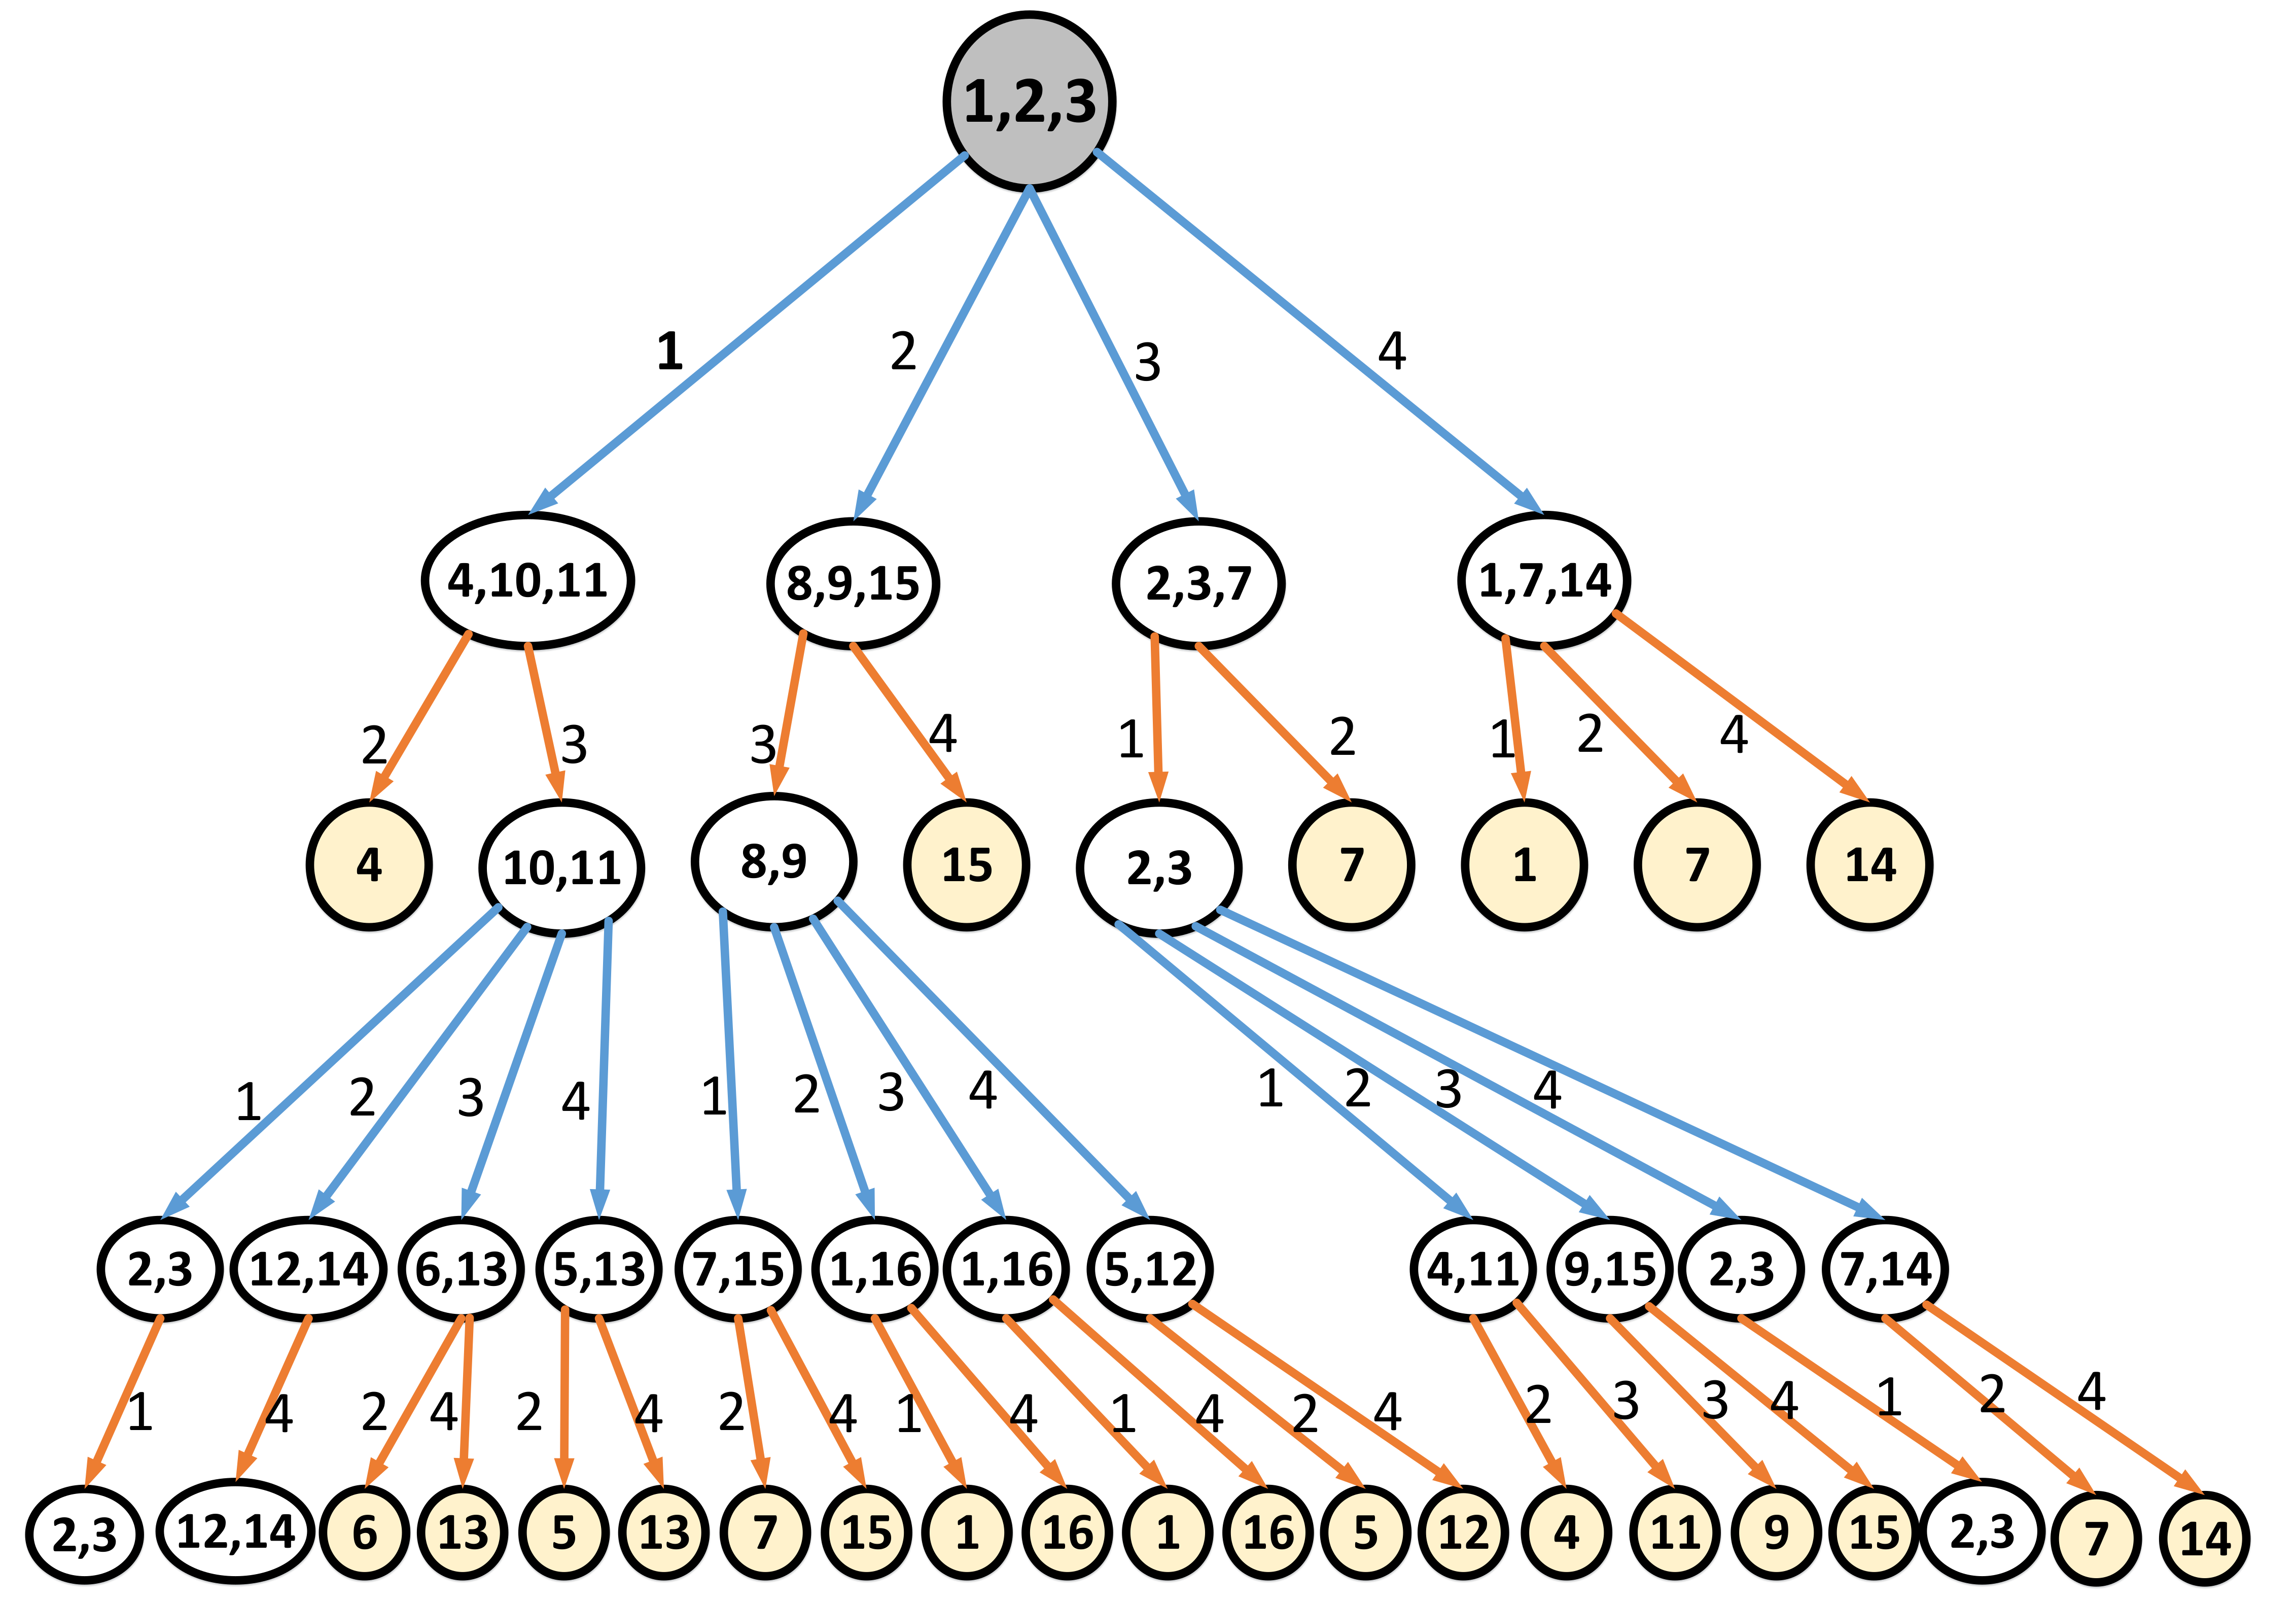
\includegraphics[scale=0.067]{figures/Fig3.png}}
	}}
      
      \caption{Branch of the super tree which represents $\{\delta_{16}^1,\delta_{16}^2,\delta_{16}^3\}$. The blue edges and orange edges show the observing output processes and deciding input processes, respectively. The yellow nodes are leaf nodes.}
      \label{fig:3}
   \end{figure}

At the beginning we infer that the possible states set is $\Delta_N$, thus the root node of the super tree is $\Delta_N$. When the cardinal number of the possible states set turns into $1$, we can determine the state of \BCN. Therefore, the leaf nodes of the super tree are the nodes with cadinal number $1$. We observe the output of \BCN\ to infer the possible states set of \BCN\ at first. After that, we decide the input and infer the new possible states set. We alternately observe the output and decide the input untill we can determine the state of {\em BCN}. Therefore we use $D\left(S',\varepsilon, O'\right)$ to find son nodes for every $S'$ in $2k+1$ layer, and using $D\left(S',I',\varepsilon\right)$ to find son nodes for every $S'$ in $2k+2$ layer. The formula $|D\left(S',\varepsilon, O'\right)|>0$ ensures the node $D\left(S',\varepsilon, O'\right)$ has meaning. The formula $|D\left(S',I',\varepsilon\right)|=|S'|$ guarantee we can determine the state of \BCN\ in the end. 

For example, the Fig.\ref{fig:3} show branch of the tree which represents $\{\delta_{16}^1,\delta_{16}^2,\delta_{16}^3\}$. The nodes represent the states sets, the blue edges represent the observing output processes, and the orange edges represent the deciding input processes. This branch is not completed, because only the yellow nodes are the leaf nodes. If we want to find all of the ways to determine the initial state of \BCN, we have to build the complete tree for \BCN. This process takes many additional time and space overhead. Especially when there are loops in the tree, like the $\{\delta_{16}^2,\delta_{16}^3\}$ in fourth layer and the $\{\delta_{16}^2,\delta_{16}^3\}$ in fifth layer that will form a loop. In this case we can never build the complete tree, thus we need to check the existence of loops and omit it. There are also some nodes take the same states set which will also take additional overhead. For instance there are two nodes take the same states set $\{\delta_{16}^1,\delta_{16}^{16}\}$ in the fifth layer. However, it would be a lot easier if we only need to find a way to determine the initial state. For instance, when we find the leaf nodes $\delta_{16}^1$, $\delta_{16}^7$ and  $\delta_{16}^{14}$ in third layer by breadth-first algorithm, we can make sure that the states set $\{\delta_{16}^1,\delta_{16}^2,\delta_{16}^3\}$ is 1 step deterministic. After that, we use this conclusion to determine the initial state of \BCN. 
\subsection{Directed graph}
To improve the shortcomings of the way by using supertree, we proposed the way by derected graph wich takes less time and space overhead. The most difference between supertree and derected graph is that supertree is built from the root node to leaf nodes. However, the derected graph is built from smaller nodes (contain less states) to larger nodes (contain more states). There is not any repeated node in the derected graph because any node only appears once in the graph. And even there are some loops in the derected graph, the loops would not influence us to build the directed graph.

The construction algorithm of derected graph is shown in the Algorithm.\ref{alg:1}. The algorithm to build nodes used in the Algorithm.\ref{alg:1} is shown in the Algorithm.\ref{alg:2}.

\begin{algorithm}[h]
\caption{Algorithm to construct the directed graph of \BCNs}
\begin{algorithmic}[1]
\REQUIRE 
The algebraic forms of \BCN
\ENSURE  
The directed graph of \BCN
\STATE Define a int variable $k=1$, to represent the number of states in the nodes.\
\STATE Define a boolean type variable $Ob=0$, to represent the online observability of \BCN.\
\STATE buildnode(k)
\STATE $k= k+1$
\WHILE {buildnode(k)==1}
\IF{$k==2$}
\STATE Take $\Delta_M$ as the suitable inputs set of every node with $k$ states.
\ELSE
\IF{$k>2$}
\STATE Using other nodes to find the suitable inputs set for every node with $k$ states. 
\ENDIF
\ENDIF
\FOR{every node with $k$ states}
\FOR{every input in the suitable input set of the nodes}
\STATE Checking whether this input ($I'$) can make a node ($S'$) $z$ steps. 
\STATE And then build edges for this node. 
\ENDFOR
\ENDFOR
\IF {there exist one node has not any edge connect it with other nodes}
\STATE $Ob=0$ return Ob
\ENDIF
\STATE $k= k+1$
\ENDWHILE
\STATE $Ob=1$ return Ob
\end{algorithmic}
 \label{alg:1}
\end{algorithm}

\begin{algorithm}[h]
\caption{Algorithm to build nodes with $k$ states}
\begin{algorithmic}[1]
\REQUIRE 
The number of states in the nodes $p$
\ENSURE  
The nodes with $p$ states
\STATE int buildnode(int p)
\STATE  \{ 
%\dfSTATE $p=p+1$\
\STATE  Try to build all the nodes with $p$ states, the corresponding outputs states are the same.\
\STATE  Classify these nodes by their corresponding outputs.
\IF{Failed to build} 
\STATE  return 0;
\ELSE 
\STATE Sort the states in the nodes, and then sort the nodes. %(For example, the nodes $\{\delta_{16}^1,\delta_{16}^2\}$, $\{\delta_{16}^1,\delta_{16}^3\}$ and $\{\delta_{16}^2,\delta_{16}^3\}$ shown in {\em Fig.\ref{fig:4}}. )
\STATE return 1;
\ENDIF 
\STATE \}
\end{algorithmic}
 \label{alg:2}
\end{algorithm}

Some details in Algorithm.\ref{alg:1} and Algorithm.\ref{alg:2} are as follows:
\begin{itemize}
 \item Sort the states in the nodes, and then sort the nodes: For example, the nodes $\{\delta_{16}^1,\delta_{16}^2\}$, $\{\delta_{16}^1,\delta_{16}^3\}$ and $\{\delta_{16}^2,\delta_{16}^3\}$ shown in Fig.\ref{fig:4}. 
  \item Use other nodes to find the suitable inputs set for nodes with $k$ states: For example, we can search inputs sets which make $\{\delta_{16}^4,\delta_{16}^5,\delta_{16}^6\}$, $\{\delta_{16}^5,\delta_{16}^6,\delta_{16}^7\}$ and $\{\delta_{16}^4,\delta_{16}^7\}$ $k$ steps deterministic at first. After that, take the intersection of these sets to be the suitable inputs set of $\{\delta_{16}^4,\delta_{16}^5,\delta_{16}^6,\delta_{16}^7\}$. 
  \item Check whether an input ($I'$) can make a node ($S'$) $z$ steps deterministic: According to the order determined in previous steps, we check every node in order. If for one input $I'$ which belongs to suitable inputs set of the states set $S'$ implies $|D\left(S',I',\varepsilon\right)|<|S'|$, we can make sure the $I'$ is a wrong input. Else if for all $O' \in \Delta_Q$ and $|D\left(S',I',O'\right)|>0$, the $D\left(S',I',O'\right)$ is $z$ steps deterministic then $I'$ is a right input. Therefore, we can connect the node $S'$ to all nodes $D\left(S',I',O'\right)$ with directed edges. The colour of directed edges represent its corresponding input. Else if there exist $O' \in \Delta_Q$ and we can not make sure whether $D\left(S',I',O'\right)$ is $z$ steps deterministic, we check it in the next round. 
\end{itemize} 

According the construction process, we have the definition of directed graph.
\begin{definition}[Directed Graph]
For every node $S_j$ in the directed graph, the $S_j$ is $k$ stepes deterministic. For every distinct two $s_a, s_b \in S_j$ we have $Hs_a=Hs_b$. If $|S_i|=1$ there are not edge from it to other nodes, else if there are exist one edge $I'$ from it to one nodes then there exist $p$ ($p\ge 1)$ edges contain $I'$ from it to nodes $S_1,\ldots,S_p$ that \[|S_j|= |S_1|+,\ldots,|S_p|\] and \[D\left(S_j,I',\varepsilon\right)=S_1\vee,\ldots,\vee S_p.\]
\end{definition}

When we trying to build the directed graph for a \BCN, we check whether the nodes with less states are $k$ stepes deterministic first and then check whether the nodes with more states are $k$ stepes deterministic.  As the the nodes with less states are not $k$ stepes deterministic, the nodes with more states would not be $k$ stepes deterministic.Therefore, once we can find a node is not $k$ stepes deterministic we can know that $\Delta_N$ is not $k$ stepes deterministic and this \BCN\ is not online observable. Moreover, we can use the nodes with less states that are $k$ stepes deterministic to help us check the nodes with more states. For instance, if the node $S$ has two edges from it to two nodes $S_1$ and $S_2$, and we have $S_1$ and $S_2$ are $k$ stepes deterministic. In this case, we can make sure that the node $S$ is $k$ stepes deterministic.

Based on the definitions of existing four kinds of observability, we can also use the directed graph to determine the existing second and fourth kinds of observability. When we trying to build bottom layer and penultimate layer of the directed graph, if there are exist some nodes in penultimate layer has no edges from it to other nodes. In this case this \BCN\ is not satisfied existing second observability. When we trying to build edges for every layer, and if there exist one node whose right inputs set is not $\Delta_M$, then this BCN is not satisfied existing fourth observability.
\begin{figure}[thpb]
      \centering
      \framebox{\parbox{3in}{
		\centerline{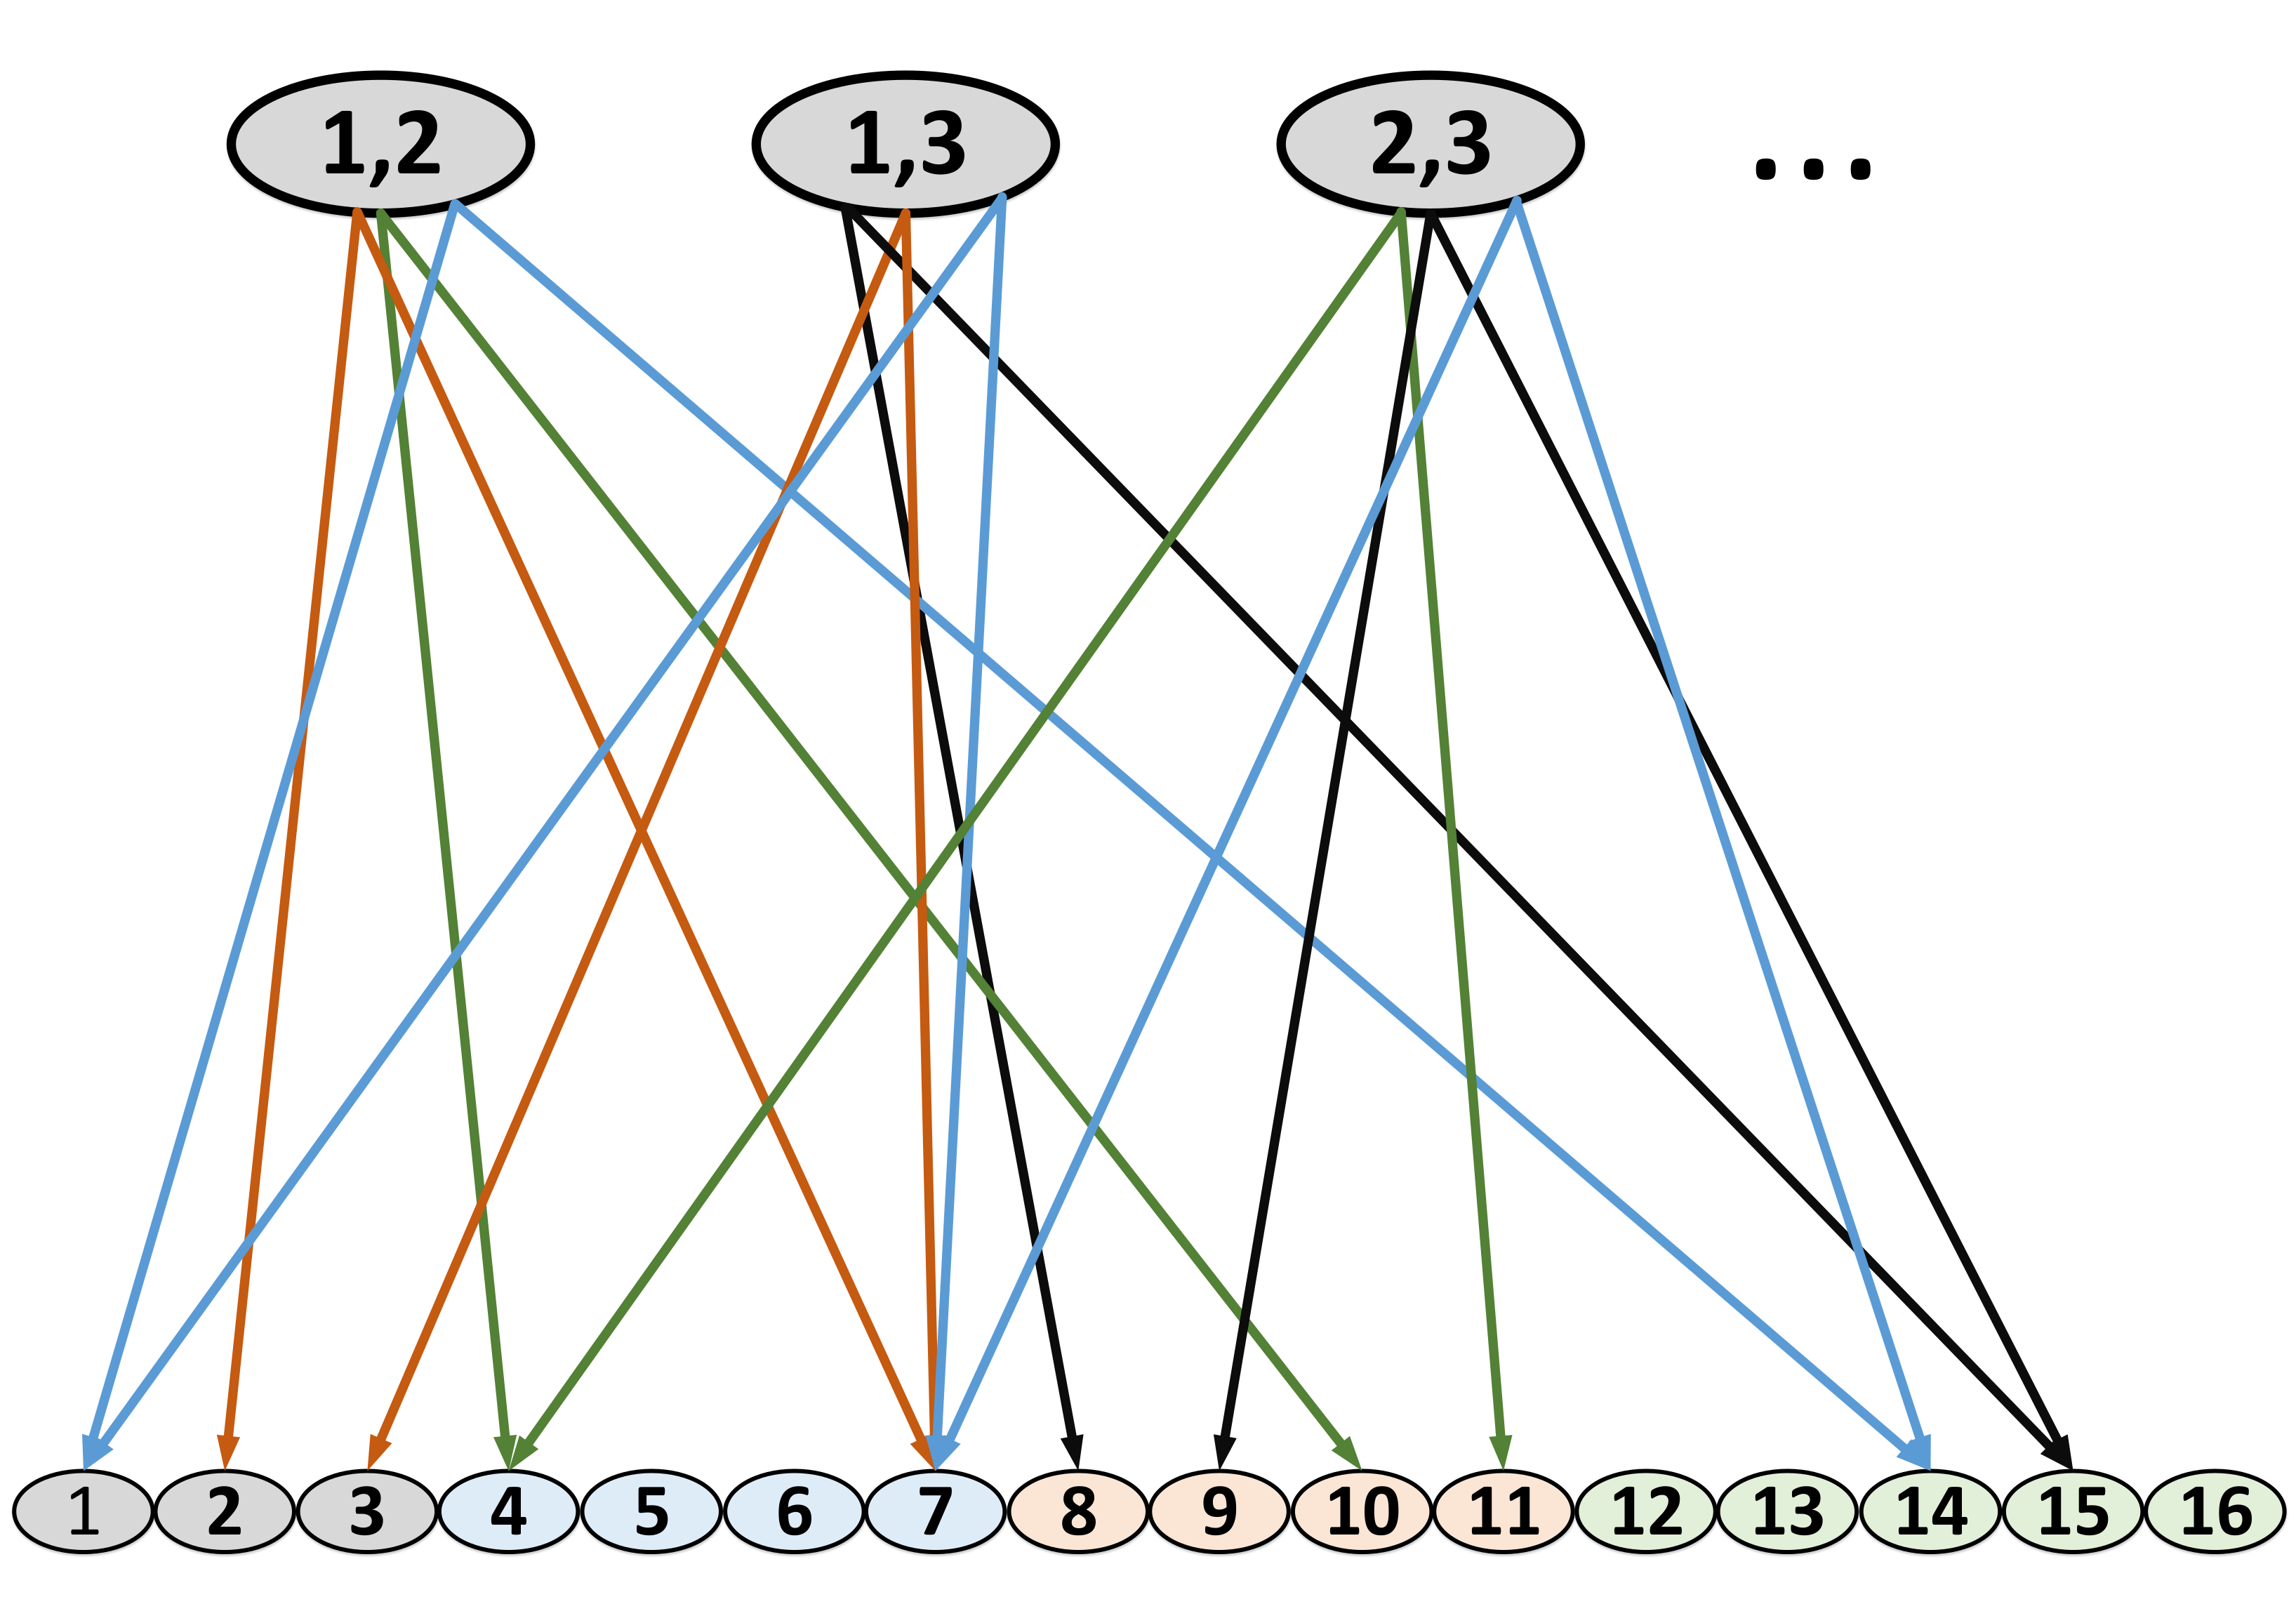
\includegraphics[scale=0.090]{figures/Fig4.png}}
	}}
      
      \caption{Part of the directed graph which represents $\{\delta_{16}^1,\delta_{16}^2\}$, $\{\delta_{16}^1,\delta_{16}^3\}$ and $\{\delta_{16}^2,\delta_{16}^3\}$. The green, black, orange, blue edges show the inputs $\delta_4^1$, $\delta_4^2$, $\delta_4^3$ and $\delta_4^4$ respectively.}
      \label{fig:4}
   \end{figure}
\subsection{Complexity analysis}
The way by the directed graph is better than by supertree, thus we analyze the complexity of it. We classify the states with their corresponding output. After that form the set of states set $\{S_1, S_2,\ldots,S_M\}$,  and every element in a states set has the same corresponding output. That is to say for each $S_j\in\{S_1, S_2,\ldots,S_M\}$ then for every $s_k\in S_j$ we have $Hs_k=\delta_{M}^j$.

Firstly, we need to calculate the upper bound of the number of the states in the directed graph nodes $k$ we have.
\begin{equation}
\begin{split}
k_{upb}= \max(|S_1|,|S_2|,\ldots,|S_M|)
\end{split}
\end{equation}
The$ k_{upb}$ is the maximum value of $|S_1|,|S_2|,\ldots,|S_M|$, because the states in the directed graph nodes should have the same corresponding output.

Secondly, we need to calculate the number of nodes with $k$ states:
\begin{equation}
\begin{split}
k_{non}= C_{|S_i|}^k+\ldots +C_{|S_p|}^k
\end{split}
\end{equation}
where $S_i\ldots,S_p\in\{S_1, S_2,\ldots,S_M\}$ and $|S_i|,\ldots,|S_p|\ge k$.

Thirdly we need to calculate the cardinal number of suitable inputs set of each node. Finally we need to calculate the time used to check each input is a right input for a node.

After completing the previous steps, calculate the complexity by layer by layer. But the cardinal number of suitable inputs set of a node depends on the cardinal number of it and the other three nodes used to find the suitable inputs set for it. And the time used to check whether an input is a right input for a node also depends on the updating rules of {\em BCNs}.

Moreover, instead of taking $\Delta_M$ as the suitable inputs set for every node in thedirected graph. We would use the other three nodes like $\{\delta_{16}^4,\delta_{16}^5,\delta_{16}^6\}$, $\{\delta_{16}^5,\delta_{16}^6,\delta_{16}^7\}$ and $\{\delta_{16}^4,\delta_{16}^7\}$ that are $k$ steps deterministic to find the suitable inputs set for a node $\{\delta_{16}^4,\delta_{16}^5,\delta_{16}^6,\delta_{16}^7\}$ with more than $2$ states. By this way we can  reduce the cardinal number of the suitable inputs set for every nodes with more than 2 states, and then reduce the time cost. 

The reason why we can use this method is that only the input which make the subset of $\{\delta_{16}^4,\delta_{16}^5,\delta_{16}^6,\delta_{16}^7\}$ $k$ steps deterministic will make the $\{\delta_{16}^4,\delta_{16}^5,\delta_{16}^6,\delta_{16}^7\}$ $k$ steps deterministic. Furthermore, using these three nodes will be a good way to cover all the subset with cardinal number $2$ of $\{\delta_{16}^4,\delta_{16}^5,\delta_{16}^6,\delta_{16}^7\}$. That is to say every subset $s_k$ with cardinal number $2$ belongs to $\{\delta_{16}^4,\delta_{16}^5,\delta_{16}^6,\delta_{16}^7\}$ will belongs to $\{\delta_{16}^4,\delta_{16}^5,\delta_{16}^6\}$, $\{\delta_{16}^5,\delta_{16}^6,\delta_{16}^7\}$ or $\{\delta_{16}^4,\delta_{16}^7\}$. This conclusion can help us to select the nodes we need when we seek the suitable inputs set for a node. But it is hard to analyze the complexity of this method, and it makes the complexity analysis of the way by directed graph harder.

Therefore, it is hard to give a accurate complexity of the algorithm without the complete imformation of \BCNs. We may finish this job in the furture, and we will try to use real example to do complexity analysis.
%Because the states in a nodes will have the same corresponding output, so we have the upper bound of the number of the states in a directed graph nodes $k$: We classify the states with their corresponding output and form the set of states with the same corresponding output, the greatest cardinal number of these set would be the upper bound of $k$. 